\subsection{Performance Evaluation across Dimensions}

\begin{figure}[h]
\centerline{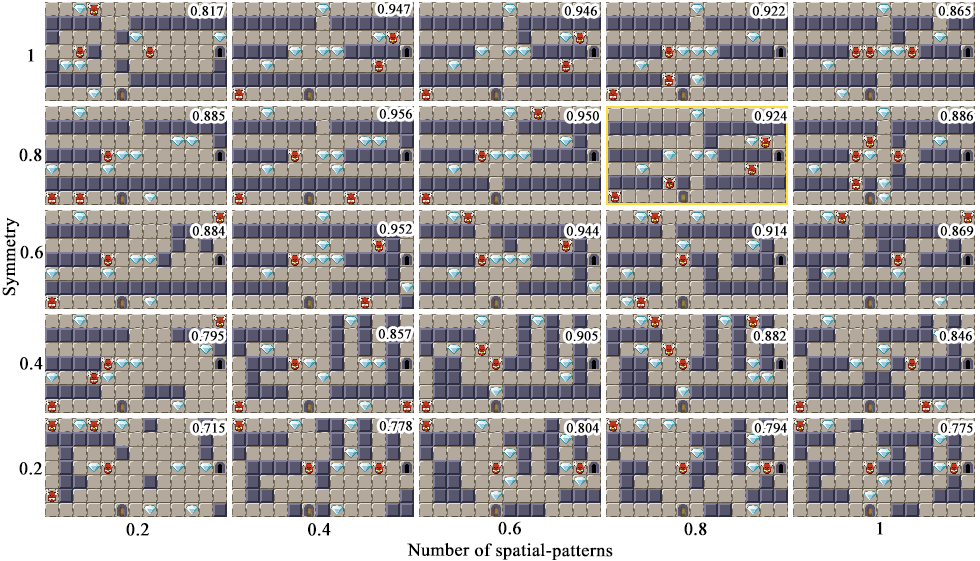
\includegraphics[width=0.48\textwidth]{figures/figure3.png}}
\caption{Rooms at generation $2090$ targeting Number of spatial-patterns (X) and Symmetry (Y). Each cell displays (top-right) the fitness of the optimal individual in its related feasible population. }
\label{figs:patt_sym}
\end{figure}

First, we ran a set of experiments to test the results from the IC MAP-Elites using all possible combinations of the available dimensions using two dimensions at a time. All experiments were run using $13\times7$ rooms, the same room size as in \emph{The Binding of Isaac}~\cite{p6mcmillen_binding_2011}, a representative example of a dungeon-based adventure game. In each experiment, the initial population was set to $1000$ mutated individuals distributed in feasible and infeasible populations in all cells which were set to a maximum capacity of $25$ individuals each. IC MAP-Elites ran continuously, and every $100$ generations rendered the elites of each cell. At each generation, it selected $5$ parents per population among uniformly random chosen cells. Offspring were always produced through a two-point crossover and had a 30\% chance of being mutated, which would randomly alter one tile in the level.

\Cref{figs:patt_sym} shows a grid containing the best found suggestions at generation $2090$, while aiming for number of spatial-patterns at the X-axis and symmetry at the Y-axis with a granularity of $5$. Each cell displays the optimal individual of the feasible population under a given pair of dimension values. The fitness score is displayed on the cells' top-right corner.

The fitness evaluation in IC MAP-Elites is quite lightweight in terms of computational cost, which enables the grid of suggestions to be completed in a matter of seconds. This is of principal importance for successfully implementing continuous evolution, so that the influence of each manual change in the edited rooms is reflected in the suggestions almost instantly. %The feeling of immediacy is further increased through updating cells as soon as a new optimal individual is produced and incorporated to the cell’s underlying feasible population.

Results in \Cref{figs:patt_sym} are representative of the good quality diversity solutions produced by EDD. The average fitness across elites is $0.872$, and the highest fitness is $0.956$ (cell $[0.4,0.8]$). No two rooms are the same. As intended, high levels of symmetry are displayed in the upper rows, gradually decreasing towards the bottom row. Similarly, rooms in the leftmost column contain lower amounts of spatial patterns, increasing towards the rightmost column. Lower amounts of spatial patterns translate into more open rooms with almost no corridors and one or two large adjacent chambers (as in cell $[0.2, 0.2]$), as opposed to highly pattern filled rooms that comprise intricate pathways converging at one or two small chambers (cell $[1, 0.2]$). 

Fitness values show that some dimension combinations are harder to optimize than others, so that the whole grid depicts a gradient landscape of the compatibility between each pair of dimensions. The bottom-left corner shows difficulties producing symmetric rooms with low amounts of spatial patterns, as opposed to rooms with many corridors (upper-right corner), which seem to favor the generation of symmetrical structures.% The bottom row shows that aiming for low symmetry generally produces slightly less optimal results, whereas the top row shows that corridors are the most favorable spatial pattern for building symmetric rectangular rooms.

Additional similar experiments can be found in~\cite{p6alvarez2019empowering}, where we combined other pairs of dimensions and analyzed and discussed the correlation and limitations found in them. However, in the following section, we present an extension of those evaluations through a more exhaustive and in-depth assessment of IC MAP-Elites.

% In~\cite{p6alvarez2019empowering}, we presented similar additional experiments combining other pairs of dimensions, analyzing and discussing the correlation and limitations found in them. However, in the following section we present an extension of those evaluations through a more exhaustive and in-depth assessment of IC MAP-Elites.

% Additional experiments were carried out combining other pairs of dimensions. The complete results can be found in \cite{p6alvarez2019empowering}, together with their analysis and discussion in terms of the existing correlations found between each pair of dimensions.%, as well as the effects of integrating the MAP-Elites approach into a continuously evolving environment.

% \begin{figure}[!t]
% \centering
% \includegraphics[width=2.5in]{Figures/Expressive-range/expressive_range-SIMILARITY_SYMMETRY.png}
% \caption{Example of expressivity range (5000 generations)}
% \label{fig_sim}
% \end{figure}
